%\documentclass[0-main.tex]{subfiles}
%\begin{document}

\section{Experiments}\label{sec:exp}
We evaluate \hirl with a series of standard RL benchmarks and in a physical experiment on the da Vinci surgical robot.

\subsection{Methodology}
All of the experimental scenarios followed a similar pattern: (1) start with an RL problem with a delayed reward, (2) generate $N$ demonstration trajectories with motion planning in simulated scenarios and kinethestic demonstration in the physical experiments, (3) apply \hirl, (4) evaluate the performance of the policy as a function of the $I$ iterations.
For all convergence curves presented, we show the probability of task success as a function of the number of RL iterations.
For convergence rate, we measure the Area Under Curve of the learning curve (i.e., cumulative expected reward over the learning epoch).

\noindent The algorithms considered in the experiments are:
\begin{enumerate}[
    topsep=0pt,
    noitemsep,
    % partopsep=1ex,
    % parsep=1ex,
    leftmargin=*,
    % itemindent=3ex
    ]
    \item \textbf{Q-Learning: } This applies a Q-Learning algorithm with the same hyper-parameter setting as \hirl. 
    \item \textbf{Pure MaxEnt-IRL: } Given $N$ demonstrations this learns a reward using MaxEnt-IRL and no hierarchical structure. Then, it applies Q-Learning with the same hyper-parameter setting as \hirl until convergence. (Only Phase II and III)
    \item \textbf{SVM: } Given $N$ demonstrations this learns a policy using a multi-class SVM classifier. There is no further learning after training. (Directly to Policy)
    \item \textbf{\HIRL (Model-Based) and \HIRL (Model-Free)} 
\end{enumerate}

\iffalse
\subsection{GridWorld}
We start with an example of to illustrate how delayed rewards in sequential tasks pose a challenge in RL.
We modified a variant of one of the canonical RL domains in RLPy~\cite{RLPy}, GridWorld, to illustrate how \hirl addresses problems of sequentiality (Figure~\ref{exp:gweasy1}). 
% This experiment intuitively illustrates the challenge of sequential rewards in RL.
RL algorithms find an optimal stationary policy, i.e., a time-invariant function between states and actions.
Even straight-forward sequential dependencies can introduce situations where any successful policy needs to take two different actions in the same state, depending on stage of the task.

We constructed a grid world with two goal states denoted by ``0'' and ``1'' separated by a narrow passage to illustrate the challenge of sequential dependency.
The robot can only receive the reward at ``1'' if it has previously reached ``0".
In the $(x,y)$ state-space, the robot does not learn a correct stationary policy since at some states the optimal action depends on knowing whether ``0'' has been reached.
Thus, directly applying RL to the this problem results in an algorithm that converges to finding only one reward.

\hirl can address this problem. We first collect 3 demonstrations of manually traced out paths that go to ``0'' and then ``1''.
The robot needs to know which phase of the task it is in and during this stage which reward point is the focus.
\hirl learns three segments, and using a reward constructed with \hirl and an augmented state-space, Q-Learning converges to find both rewards.
Since GridWorld has known dynamics, we used the model-based variant of of \hirl.

\begin{figure}[t]
\centering
 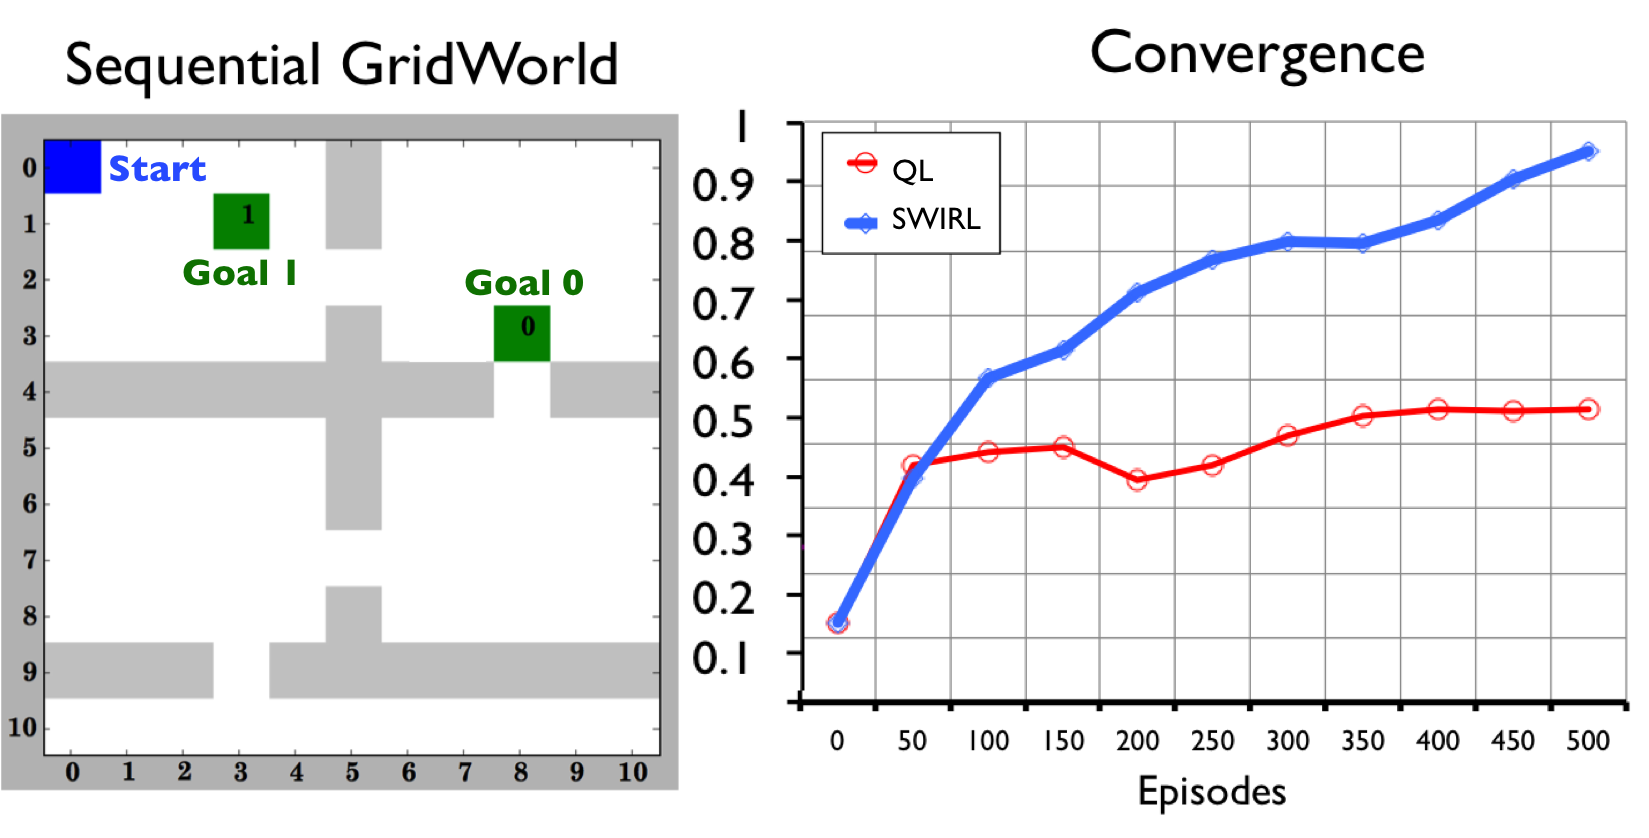
\includegraphics[width=0.8\columnwidth]{exp/wafr-gridword-1.png}
 \caption{GridWorld: the two goal states must be reached in sequence to receive a reward. RL algorithms find an optimal stationary policy, i.e., a time-invariant function between states and actions. In this case, Q-Learning fails to find a successful policy since a non-stationary decision is required (go right if in stage 1 of the task, go left if in stage 2). \hirl addresses this problem by segmenting the task and applying RL with an augemented state-space.\label{exp:gweasy1}}
\end{figure}
\fi

\subsection{Parallel Parking}\label{exp:pp}
We constructed a parallel parking scenario for a robot with non-holonomic dynamics and two obstacles. The robot can control its speed ($\|\dot{x}\|+\|\dot{y}\|$) and heading ($\theta$), and observe its x position, y position, orientation, and speed in a global coordinate frame.
If the robot parks between the obstacles, i.e., 0 velocity within a $15^\circ$ tolerance, the task is a success and the robot receives a reward of $1$. 
The robot's dynamics are noisy and with probability 0.1 will randomly add or subtract $5^\circ$ degrees from the steering angle.
If the robot collides with one of the obstacle or does not park in 200 timesteps the episode ends. 
The baseline approach is modeling the entire problem as an MDP with a quadratic reward function at the target state (where the robot parks).
For comparison, we use this reward function for Q-Learning and infer a quadratic reward function using MaxEnt-IRL.
We call this domain Parallel Parking with Full Observation (PP-FO) (see Figure~\ref{exp:rcsegmentation}).

Next, we made the  Parallel Parking domain a little harder. We hid the velocity state from the robot, so the robot only sees $(x,y,\theta)$. As before, if the robot collides with one of the obstacle or does not park in 200 timesteps the episode ends.
We call this domain Parallel Parking with Partial Observation (PP-PO).

We generated 5 demonstrations using an RRT motion planner (assuming deterministic dynamics) and applied \hirl to learn the segments.
Figure \ref{exp:rcsegmentation} illustrates the demonstrations and the learned segments. There are two intermediate goals corresponding to positioning the car and orienting the car correctly before reversing.

\vspace{-15pt}
\subsubsection{Performance}\label{exp:ppc} 
In the fully observed problem, compared to MaxEnt-IRL, the model-based \hirl converges to a policy with a 60\% success rate with about 3x fewer time-steps.
The gains for the model-free version are more modest with a 50\% reduction.
The supervised policy learning approach achieves a success rate of 47\% and the baseline RL approach achieves a success rate of 36\% after 250000 time-steps.

The baseline Q-Learning approach directly tries to learn a sequence of actions to minimize the quadratic cost around the target state. 
This leads to a lot of exploration since the robot must first make ``negative'' progress (pulling forward). 
\hirl improves convergence since it structures the exploration through the segmentation.
The local reward functions are better shaped to guide the car towards its short term goal.
This focuses the exploration on solving the short term problem first.
MaxEnt-IRL mitigates some of the problems since it rewards states based on their estimated cost-to-go, but as the time-horizon increases the estimates of this become nosier--leading to worse performance (see technical report for a characterization~\cite{krishnan2016hirl}).

In the partial observation problem (PP-PO), there is no longer a stationary policy that can achieve the reward.
The techniques that model this problem with a single MDP all fail to converge.
The learned segments in \hirl help disambiguate dependence on history.
After 250000 time-steps, the policy learned with model-based \hirl has a 70\% success rate in comparison to a <10\% success rate for the baseline RL, MaxEnt-IRL, and 0\% for the SVM.

Finally, we explore how well the constructed rewards transfer if the dynamics are perturbed in the fully observed setting.
We expect MaxEnt-IRL to transfer well because it learns a delayed reward, which tends to encode success conditions and not task-specific details.
After constructing the rewards, we randomly perturbed the system dynamics by introducing a bias towards turning left.
We find that the model-based \hirl technique transfers to this domain comparably to MaxEnt-IRL until the task is so different that the sub-goals learned with \hirl are no longer informative.
The model-free \hirl algorithm converges more slowly; requiring 20\% more time-steps to converge to the same success rate. 


\begin{figure}[t]
\centering
 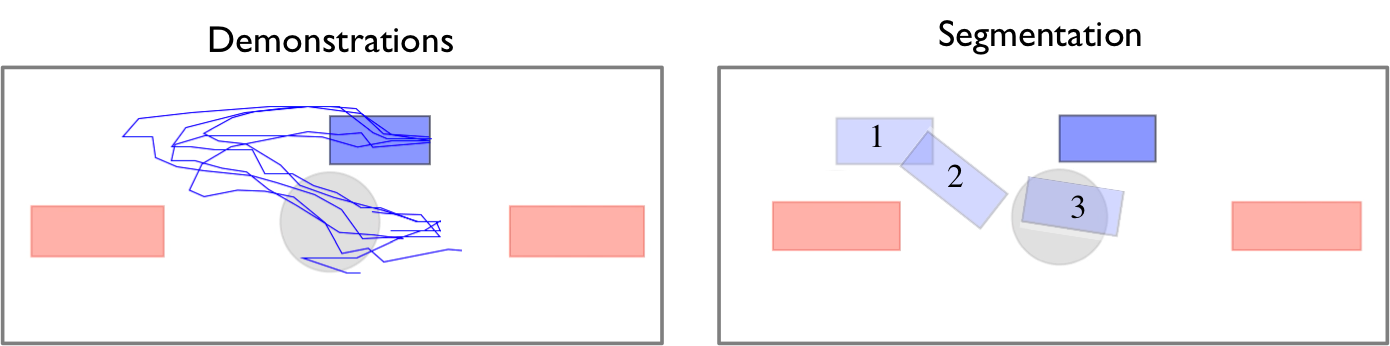
\includegraphics[width=0.8\columnwidth]{exp/rc-car-segmentation.png}
 \caption{This plot illustrates (left) the 5 demonstration trajectories for the parallel parking task, and (right) the sub-goals learned by \hirl. \label{exp:rcsegmentation}}
\end{figure}


\begin{figure}[t]
\centering
 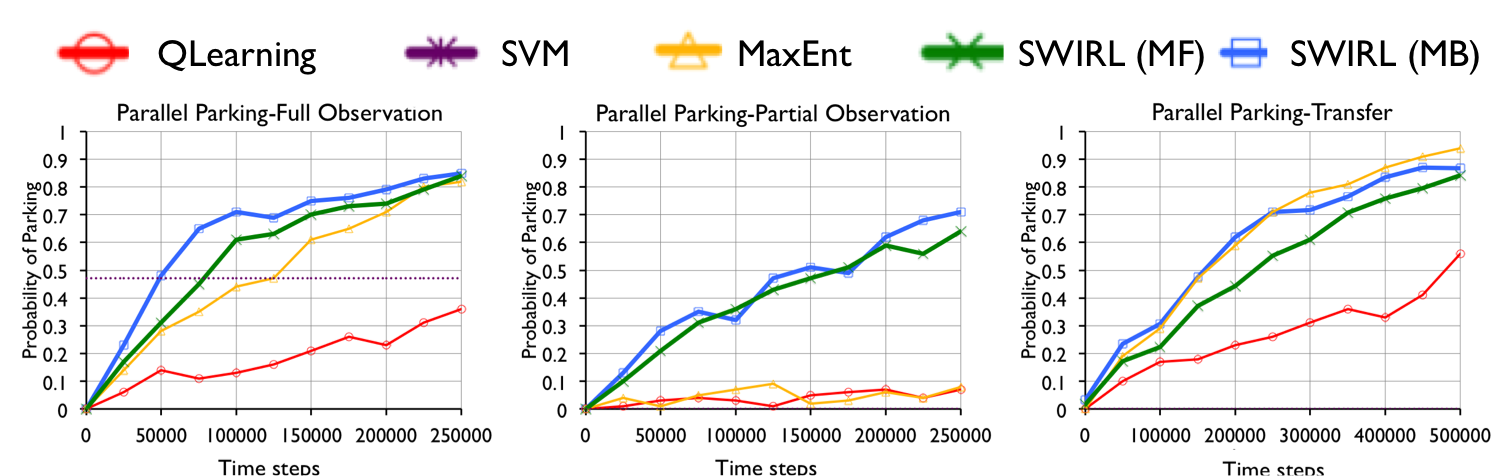
\includegraphics[width=\columnwidth]{exp/rc-convergence-1.png}
 \caption{Performance on a parallel parking task with noisy dynamics with full state observations (position, orientation, and velocity), partial observation (only position and orientation), and transfer (randomly permuting the action space).
 Success is measured in terms of the probability that the car successfully parked, and (M) denotes whether the approach used the dynamics model.
 In the fully observed case, both the model-based and model-free \hirl algorithms converge faster than MaxEnt-IRL and quickly outperforms the SVM.
 In the partially observed case, MaxEnt-IRL, Q-Learning, and the SVM fail--while \hirl succeeds.
 Both techniques also demonstrate comparable transferability to MaxEnt-IRL when the domain's dynamics are perturbed.
\label{exp:rcsegmentation-res}}
\end{figure}




\iffalse
\begin{figure}[t]
\centering
 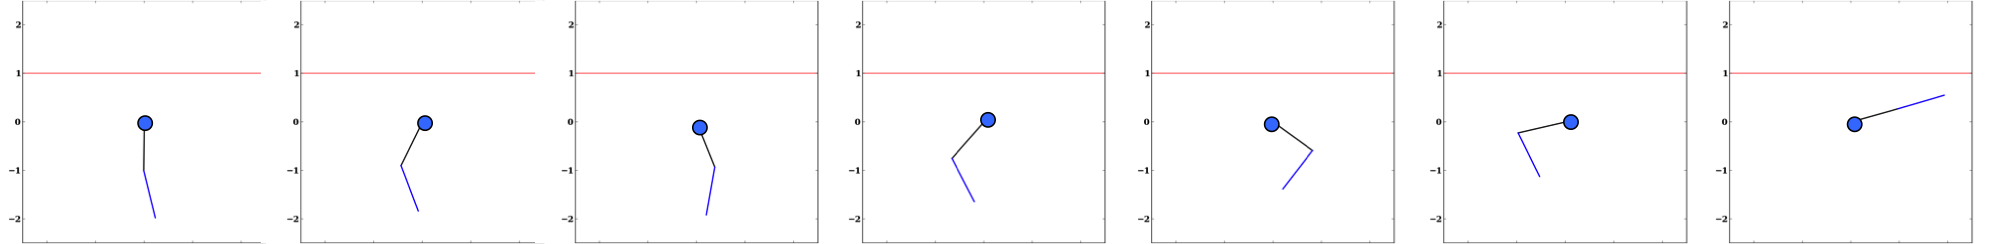
\includegraphics[width=\textwidth]{exp/segmentation-acrobot-segments.png}
 \caption{We apply \hirl to segment 5 demonstrations of Acrobot trajectories. We visualize the segments, and we find that these provide sub-goals for the robot to reach the threshold.\label{exp:acroseg} \todo{this figure isnt as useful as we would like it to be}}
\end{figure}
\fi


\begin{figure}[t]
\centering
 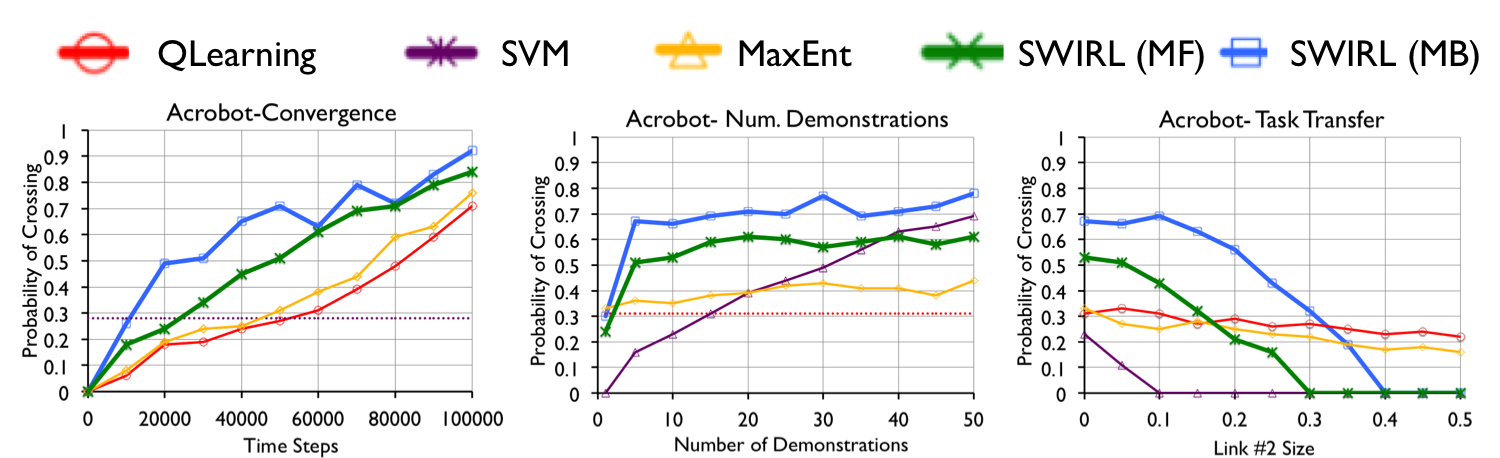
\includegraphics[width=\columnwidth]{exp/acr-convergence-1.png}
 \caption{Acrobot: We measured the performance of rewards constructed with \hirl and the alternatives. We find that \hirl (model-based and model-free) converges faster than MaxEnt-IRL, Q-Learning, and the SVM.
 Furthermore, \hirl requires less demonstrations, which we measure by comparing the performance of the alternatives after a fixed 50000 time-steps and with varied input demonstrations. 
 We also vary the task parameters by changing the size of the second link of the pendulum and find that the learned rewards are robust to this variation (as before comparing the performance of the alternatives after a fixed 50000 time steps). MaxEnt-IRL shows improved transfer performance since once the task has changed enough the segments learned during the demonstrations may not be informative and may even hurt performance if they are misleading. 
 \label{exp:acsegmentation-res2}}
\end{figure}

\subsection{Acrobot}\label{exp:acrobot}
This domain consists of a two-link pendulum with gravity and with torque controls on the joint. The dynamics are noisy and there are limits on the applied torque. The robot has 1000 timesteps to raise the arm above horizontal ($y=1$ in the images). If the task is successful and the robot receives a reward of $1$. 
Thus, the expected reward is equivalent to the probability that the current policy will successfully raise the arm above horizontal.
We generated $N=5$ demonstrations for the Acrobot task and applied segmentation. 
These demonstrations were generated by training the Q-Learning baseline to convergence and then sampling from the learned policy.
%We visualize the learned segments in Figure \ref{exp:acroseg}, which can be seen to qualitatively describe a successful path.
In Figure \ref{exp:acsegmentation-res2}, we plot the performance of the all of the approaches.
We include a comparison between a Linear Multiclass SVM and a Kernelized Multiclass SVM for the policy learning alternative.
In this example, we find that applying MaxEnt-IRL does not improve the convergence rate.
For this state-space, MaxEnt-IRL merely recovers the reward used in the original RL problem.
On the other hand, added segments using \hirl improve convergence rates.

% the \hirl approaches add segments making it easier to converge.

We also vary the number of input demonstrations to \hirl and find that it requires fewer demonstrations than policy learning and MaxEnt-IRL to converge to a more reliable policy.
It takes about 10x more demonstrations for the supervised learning approach to reach comparable reliability.
Finally, we find that \hirl does not sacrifice much transferability.
We learn the rewards on the standard pendulum, and then during learning we vary the size of the second link in the pendulum.
We plot the success rate (after a fixed 50000 steps) as a function of the increase link size.
\hirl is significantly more robust than supervised policy learning to the increase in link size and has a significantly higher success rate than IRL for small perturbations in link size. 

\subsection{Summary of Simulated Experiments}
Table \ref{tab:my_label} summarizes the results of our experiments in terms of convergence rate and maximum attained reward on the Parallel Parking domain (with and without partial observation), Acrobot domain, and additional experiments using variants of GridWorld.
GridWorld is a two-room map where the robot has to reach two target states in sequence to get the full reward.
GridWorld-2 is a substantially harder map with ``pits'' (i.e., instant failure if reached).
The Two-Bridges domain is another GridWorld based environment in which there is a short ``unsafe'' path between start and goal and a longer ``safe'' path (which is actually the optimal solution). Please refer to the arXiv report\,\cite{krishnan2016hirl} for more details.

\begin{table*}[ht]
\footnotesize
    \centering
    \caption{This table summarizes the convergence rate (\textbf{AUC}) and max reward (\textbf{MAX}) attained by a Q-learning robot using the alternatives after a fixed number of iterations. 
    \label{tab:my_label}}
    \resizebox{\linewidth}{!}{% put in textwidth
    \begin{tabular}{r||r|r|r|r|r|r|r|r|r|r|r|r}
    \hline
        \rowcolor[HTML]{CBCEFB}
         &  \multicolumn{2}{c|}{GridWorld}&
         \multicolumn{2}{c|}{GridWorld-2}& \multicolumn{2}{c|}{Two-Bridges} & %\multicolumn{2}{c|}{MW}&
         \multicolumn{2}{c|}{PP(FO)}
         & \multicolumn{2}{c|}{PP(PO)}& \multicolumn{2}{c}{Acrobot} \\ %\multicolumn{2}{c|}{Pinball}\\
    \hline
       & Max & AUC & Max & AUC & Max & AUC & Max & AUC & Max & AUC & Max & AUC\\
    \hline  \hline
        \rowcolor[HTML]{E0E0E0}
        Q-Learning & $0.984$ & $10.976$ &$0.861$  & $15.440$& $1.090$ & $16.270$& $0.911$ &$109.76$ & $0.311$ &$27.419$ & $0.944$ &$3.447$\\
%    \hline
%        Sliding & $0.322$ & $-4.322$ & $-0.190$ & $-6.200$ & $1.672$ & $18.312$ & $0.764$ &$69.664$ & $0.464$ &$51.103$ & $0.931$ &$2.214$\\
        MaxEnt-IRL & $0.987$ & $299.556$ & $0.861$ & $16.956$ & $0.759$ & $16.270$ & $0.950$ &$299.556$ & $0.444$ &$33.128$ & $0.920$ &$44.111$\\
        \rowcolor[HTML]{E0E0E0}
        \hirl (MF) & $1.830$  & $322.125$ & $1.764$ & $14.070$ & $\mathbf{1.751}$& $\mathbf{18.953}$ & $\mathbf{0.991}$ &$164.127$ & $0.934$ &$123.115$ & $0.906$ &$20.935$\\
        
        \hirl (MB) & $\mathbf{1.835}$ & $\mathbf{514.113}$ & $\mathbf{1.827}$ & $\mathbf{28.632}$ & $1.577$ & $17.141$ & $0.965$ & $\mathbf{514.113}$ & $\mathbf{0.958}$ & $\mathbf{333.897}$ & $\textbf{0.987}$ &$\textbf{65.512}$\\
    \hline
    \end{tabular}
    }
\end{table*}
\vspace{-10pt}

\subsection{Physical Experiments with the da Vinci Surgical Robot}
In physical experiments, we apply \hirl to learn to cut along a marked line in gauze similar to Murali et al.~\cite{murali2015learning}.
This is a multi-step problem where the robot starts from a random initial state, has to move to a position that allows it to start the cut, and then cut along the marked line.
We provide the robot 5 kinesthetic demonstrations by positioning the end-effector and then following various marked straight lines.
The state-space of the robot included the end-effector position $(x,y)$ as well as a visual feature indicating its pixel distance to the marked line $(pix)$.
This visual feature is constructed using OpenCV thresholding for the black line.
Since the gauze is planar, the robot's actions are unit steps in the $\pm x, \pm y$ axes.
Figure\,\ref{exp:dvrk1} illustrates the training and test scenarios.

As expected, the algorithm identifies two consistent changes in local linearity corresponding to the positioning step and the termination.
The learned reward function for the position step minimizes $x,y,pix$ distance to the starting point and for the cutting step the reward function is more heavily weighted to minimize the $pix$ distance.
We defined task success as positioning within $1$\,cm of the starting position of the line and during the following stage, missing the line by no more than $1$\,cm (estimated from pixel distance).
Since we did not have a dynamics model, we evaluated the model-free version of \hirl, Q-Learning, and the SVM.
\hirl was the only technique able to achieve the combined task.
This is because the policy for this task is non-stationary, and \hirl is the only approach of the alternatives that can learn such a policy.

We evaluated the learned tracking policy to cut gauze.
We ran trials on different sequences of curves and straight lines. 
Out of the 15 trials, 11 were successful.
2 failed due to \hirl errors (tracking or position was imprecise) and 2 failed due to cutting errors (gauze deformed causing the task to fail).
1 of the failures was on the 4.5 cm curvature line and 3 were one the 3.5 cm curvature line.


% \begin{figure}[t]
% \centering
%  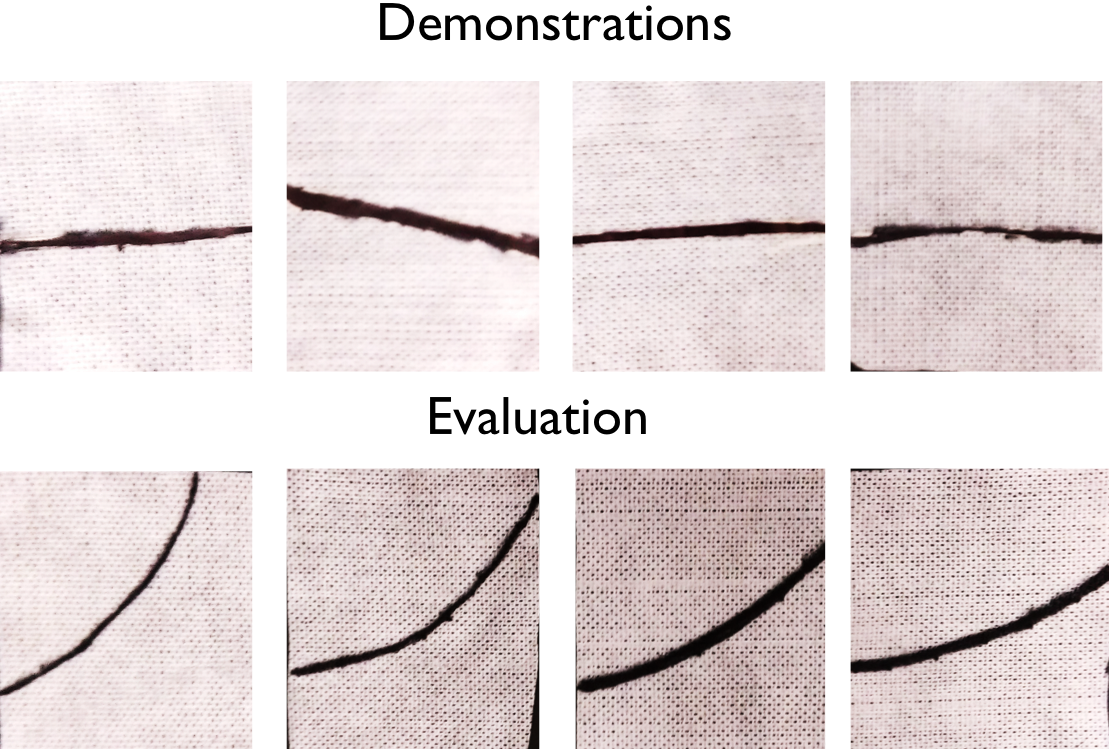
\includegraphics[width=0.7\textwidth]{exp/dvrk-demos-1.png}
%  \caption{We collected demonstrations on the da Vinci surgical robot kinesthetically. The task was to cut a marked line on gauze. We demonstrated the location of the line without actually cutting it. The goal is to infer that the demonstrator's reward function has two steps: position at a start position before the line, and then following the line. We applied this same reward to lines that were not straight nor started in exactly the same position.\label{exp:dvrk1}}
% \end{figure}

% \begin{SCfigure}[10][t]
%     \centering
%     \vspace{-0.5em}
%     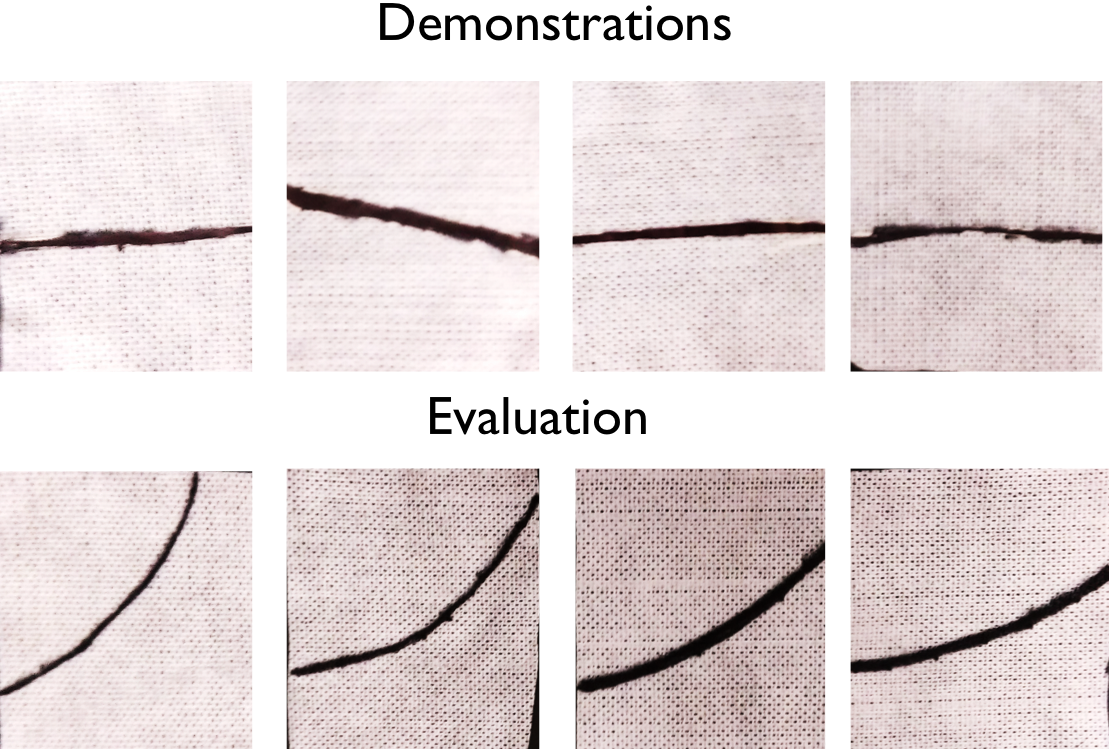
\includegraphics[width=0.5\textwidth]{exp/dvrk-demos-1.png}
%     \caption{We collected demonstrations on the da Vinci surgical robot kinesthetically. The task was to cut a marked line on gauze. We demonstrated the location of the line without actually cutting it. The goal is to infer that the demonstrator's reward function has two steps: position at a start position before the line, and then following the line. We applied this same reward to lines that were not straight nor started in exactly the same position.}
%     \label{exp:dvrk1}
%     \vspace{-1.5em}
% \end{SCfigure}


\begin{figure}[t]
\vspace{-10pt}
\centering
    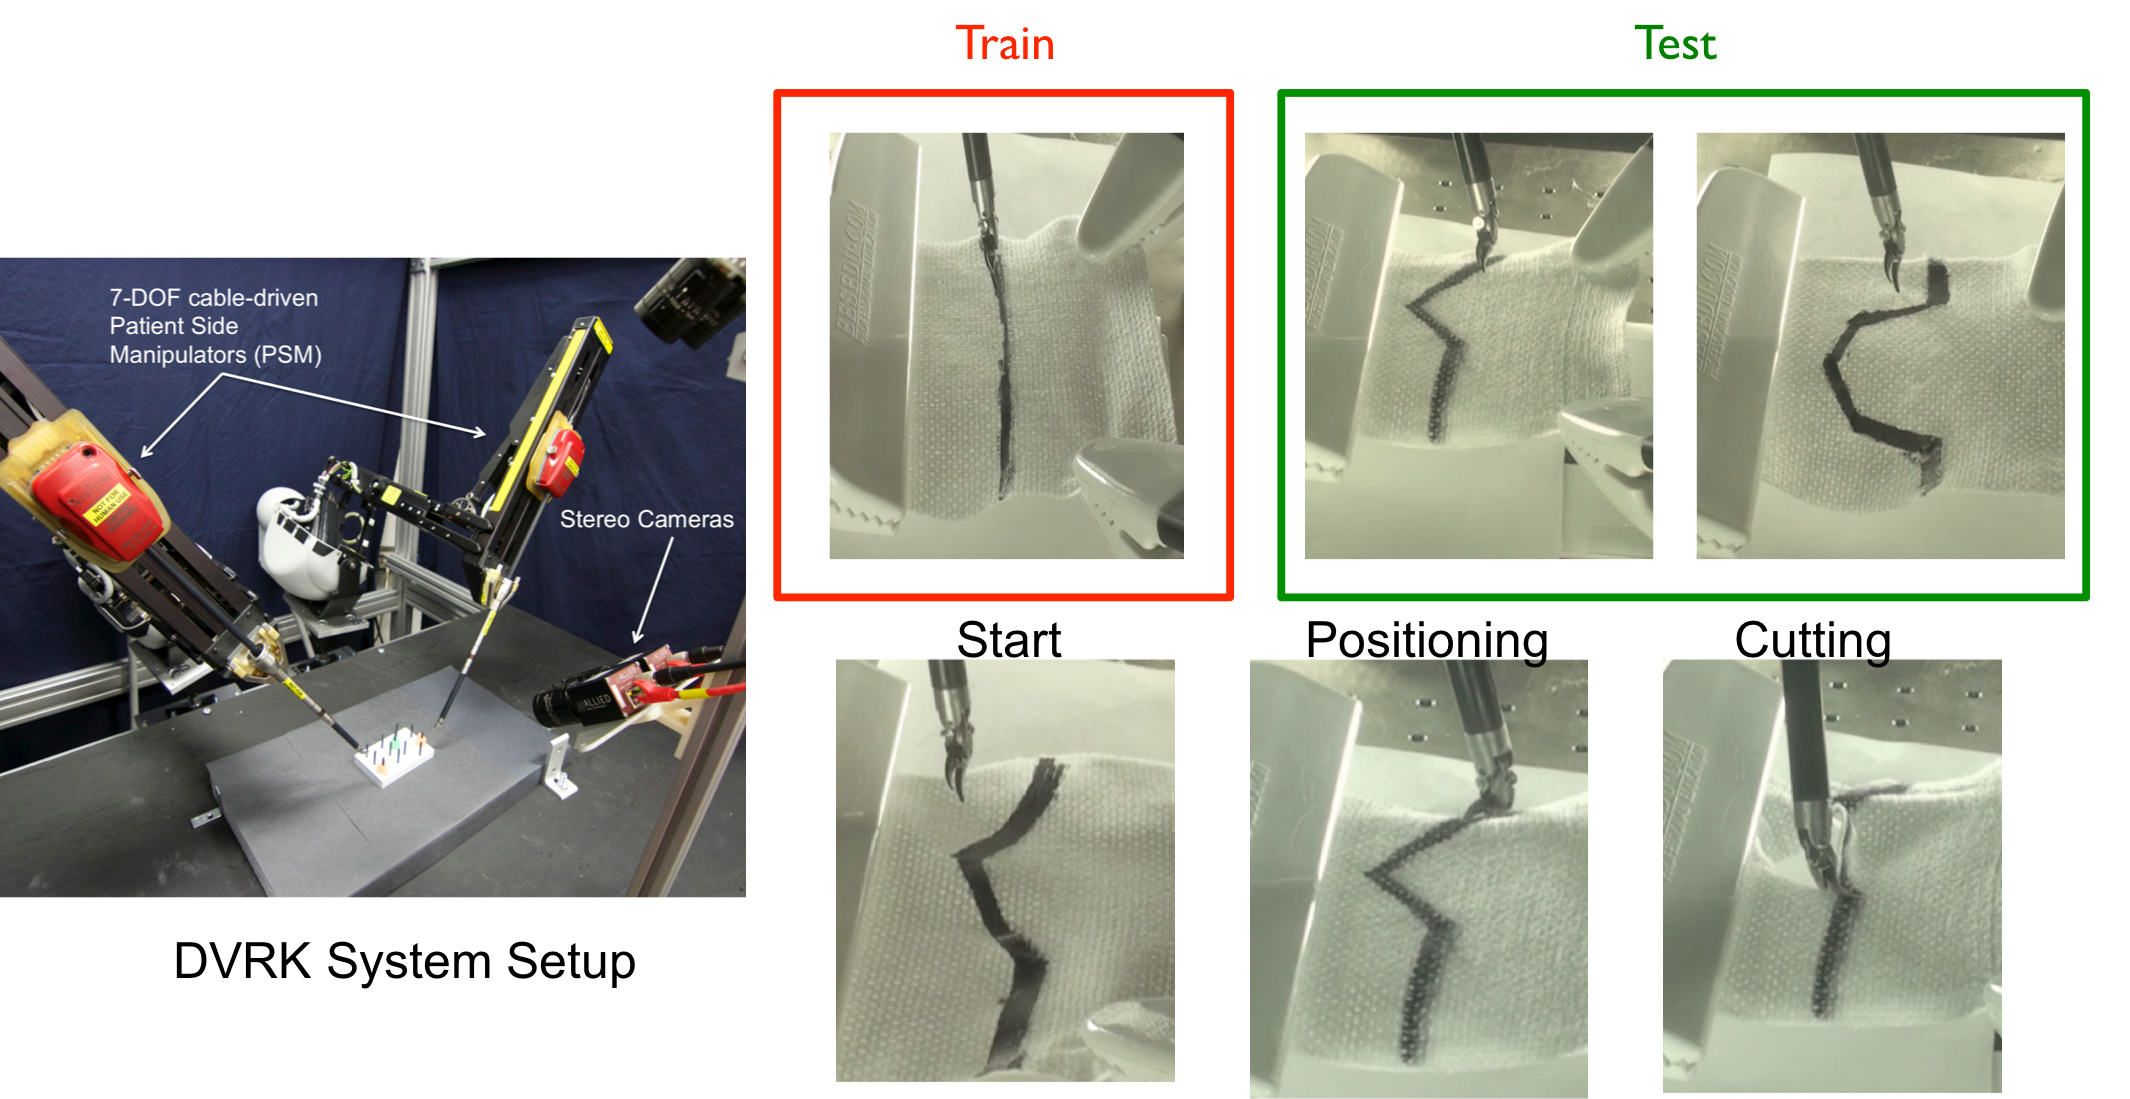
\includegraphics[width=\textwidth]{exp/dvrk-demo-2.png}
    \vspace{-10pt}
    \caption{
      We collected demonstrations on the da Vinci surgical robot kinesthetically. The task was to cut a marked line on gauze. We demonstrated the location of the line without actually cutting it. The goal is to infer that the demonstrator's reward function has two steps: position at a start position before the line, and then following the line. We applied this same reward to curved lines that started in different positions.
    }
    \label{exp:dvrk1}
% \vspace{-15pt}
\end{figure}

\begin{table}[ht]
   \scriptsize
    \centering
    \caption{With 5 kinesthetic demonstrations of following marked straight lines on gauze, we applied \hirl to learn to follow lines of various curvature. After 25 episodes of exploration, we evaluated the policies on the ability to position in the correct cutting location and track the line. We compare to SVM on each individual segment. SVM is comparably accurate on the straight line (training set) but does not generalize well to the curved lines.
    \label{dvrk:res1}}
    \vspace{-5pt}
    \resizebox{\linewidth}{!}{% put in textwidth
    \begin{tabular}{c||c|c|c|c}
    \hline
    \rowcolor[HTML]{CBCEFB} 
    Curvature Radius (cm) & SVM Pos. Error (cm) & SVM Tracking Error (cm) & \hirl Pos. Error (cm) & \hirl Tracking Error (cm) \\
     \hline \hline
    straight & 0.46 & 0.23 & 0.42 & 0.21  \\
    \rowcolor[HTML]{E0E0E0} 
    4.0 & 0.43 & 0.59 & 0.45 & 0.33 \\
    3.5 & 0.51 & {\color{red}\textbf{1.21}} & 0.56 & 0.38 \\
    \rowcolor[HTML]{E0E0E0} 
    3.0 & 0.86 & {\color{red}\textbf{3.03}} & 0.66 & 0.57 \\
    2.5 & {\color{red}\textbf{1.43}} & {\color{red}-} & 0.74 & 0.87 \\
    \rowcolor[HTML]{E0E0E0} 
    2.0 & {\color{red}}- & {\color{red}}- & 0.87 & {\color{red}\textbf{1.45}} \\
    1.5 & {\color{red}}- & {\color{red}}- & {\color{red}\textbf{1.12}} & {\color{red}\textbf{2.44}} \\
     \hline
    \end{tabular}
    }
    % \vspace{-10pt}
\end{table}
\vspace{-10pt}


Next, we characterized the repeatability of the learned policy.
We applied \hirl to lines of various curvature spanning from straight lines to a curvature radius of 1.5 cm.
Table \ref{dvrk:res1} summarizes the results on lines of various curvature.
While the SVM approach did not work on the combined task, we evaluated its accuracy on each individual step to illustrate the benefits of \hirl.
On following straight lines, SVM was comparable to \hirl in terms of accuracy.
However, as the lines become increasingly curved, \hirl generalizes more robustly than the SVM.

